\chapter{短路与用电安全}\label{ch:g7:short-circuits-safety}

你学过的每条安全规则，都可以追溯到去年曾短暂见过的一个“恶棍”：
\omterm{def:g7:short-circuits-safety:device}{短路}。本章将认真研究它——它如何发生，
为何会烧毁，以及一根不起眼的牺牲导线如何化解它，
并让家中的保险盒从一个神秘的柜子，
变成你能看懂的得力助手。

\section{恶棍的手法}

\begin{proposition}[电流偏爱省力的路径]\label{prop:g7:short-circuits-safety:effortless}
在连接同两点的两条路径之间，
电流涌向对它阻碍较小的那一条。用电器——
\omterm{def:g3:first-electric-circuit:bulb}{灯泡}、\omterm{ex:g6:circuits-and-safety:motor}{电动机}、\omterm{ex:g6:circuits-and-safety:motor}{蜂鸣器}——工作时都会阻碍电流；而
普通粗导线对它几乎没有阻碍。若为电流提供一条
裸导线旁路，电流便几乎完全离开用电器所在的路径，
转而走那条省力的路。
\end{proposition}

\begin{definition}[用电器的短路]\label{def:g7:short-circuits-safety:device}
用电器被\emph{短路}\index{短路}，是指一条导电通路
直接连接其两个\omterm{def:g3:first-electric-circuit:battery}{接线柱}，将其旁路。
电流离开该用电器——被短路的\omterm{def:g3:first-electric-circuit:bulb}{灯泡}熄灭，
\omterm{ex:g6:circuits-and-safety:motor}{电动机}停转——而电路其余部分照常工作，
此时阻碍电流的用电器少了一个。
\end{definition}

\begin{definition}[电池的短路]\label{def:g7:short-circuits-safety:battery}
最严重的情形：一条导电通路将\emph{\omterm{def:g3:first-electric-circuit:battery}{电池}}的
两个\omterm{def:g3:first-electric-circuit:battery}{接线柱}相连，路径上没有任何用电器，
电流完全不受阻碍，便化为奔涌的洪流——这股猛烈的电流
损坏\omterm{def:g3:first-electric-circuit:battery}{电池}、使导线和\omterm{def:g3:first-electric-circuit:battery}{电池}本身发热、\omterm{def:g6:water-states:changes}{熔化}
绝缘层；在市电线路上，还会引发房屋火灾。
\end{definition}

\begin{method}[安全地演示这位“恶棍”]\label{met:g7:short-circuits-safety:demo}
用一节\omterm{def:g3:first-electric-circuit:battery}{电池}和两个\omterm{def:g3:first-electric-circuit:bulb}{灯泡}\omterm{def:g4:series-circuits:series}{串联}（安全起见：\omterm{def:g3:first-electric-circuit:battery}{电池}的
推动作用很小）：
\begin{enumerate}
  \item 点亮两个\omterm{def:g3:first-electric-circuit:bulb}{灯泡}——亮度相同，
        正如\omterm{def:g4:series-circuits:series}{串联}规律所示；
  \item 现用一根普通导线接到\omterm{def:g3:first-electric-circuit:bulb}{灯泡} 2 的两个\omterm{def:g3:first-electric-circuit:battery}{接线柱}上，
        将其旁路；
  \item 观察：\omterm{def:g3:first-electric-circuit:bulb}{灯泡} 2 立即熄灭——电流已离开它——而
        \omterm{def:g3:first-electric-circuit:bulb}{灯泡} 1 变得\emph{更亮}：一个阻碍者被旁路，
        整个回路中的电流随之增强；
  \item 拿掉导线：电流重新流入\omterm{def:g3:first-electric-circuit:bulb}{灯泡} 2，
        亮度相同的状态又恢复了。
\end{enumerate}
这一实验包含三点启示：旁路的规律、
失去电流的用电器，以及增强的电流。
\end{method}

\begin{omfigure}
\begin{tikzpicture}[scale=0.9]
  \draw (0,0) to[battery1, l=电池] (0,2.8)
    to[short] (1.8,2.8)
    to[lamp, l=灯泡 1：更亮！] (4.4,2.8)
    to[lamp, l=灯泡 2：熄灭] (7.0,2.8)
    to[short] (8.4,2.8)
    to[short] (8.4,0)
    to[short] (0,0);
  \draw[very thick, omThm] (4.7,2.8) to[bend left=48] (6.7,2.8);
  \node[above, font=\small, omThm] at (5.7,3.75)
    {旁路：电流离开灯泡 2};
\end{tikzpicture}

{\small 用电器\omterm{def:g7:short-circuits-safety:device}{短路}：裸导线跨接在\omterm{def:g3:first-electric-circuit:bulb}{灯泡} 2 两端，
使\omterm{def:g3:first-electric-circuit:bulb}{灯泡} 2 的全部电流被夺走——\omterm{def:g3:first-electric-circuit:bulb}{灯泡} 2 熄灭，\omterm{def:g3:first-electric-circuit:bulb}{灯泡} 1
独自接在\omterm{def:g3:first-electric-circuit:battery}{电池}上，变得更亮。}
\end{omfigure}

\begin{example}[导线为何发热]\label{ex:g7:short-circuits-safety:heating}
电流流过时总会使其所经导线略微发热——\omterm{def:g3:first-electric-circuit:bulb}{灯泡}的发光
正是这种发热被有意利用，灯丝便是为白炽发光而设计的。
在\omterm{def:g7:short-circuits-safety:device}{短路}的奔涌中，发热变成了危险：\omterm{def:g7:short-circuits-safety:device}{短路}电流
可在数秒之内把铜导线加热到超过其塑料护套的\omterm{def:g4:changes-of-state:melting-point}{熔点}。
小尺度的预演：用导线将\omterm{def:g3:first-electric-circuit:battery}{电池}\omterm{def:g7:short-circuits-safety:device}{短路}，\omterm{def:g3:first-electric-circuit:battery}{电池}在你手中变热，
这与市电尺度上烧焦墙壁的，是同一物理规律。（
发热如何随电流增大而变化，
将在两年后，结合电功率一章，如实加以测定。
）
\end{example}

\begin{omfigure}
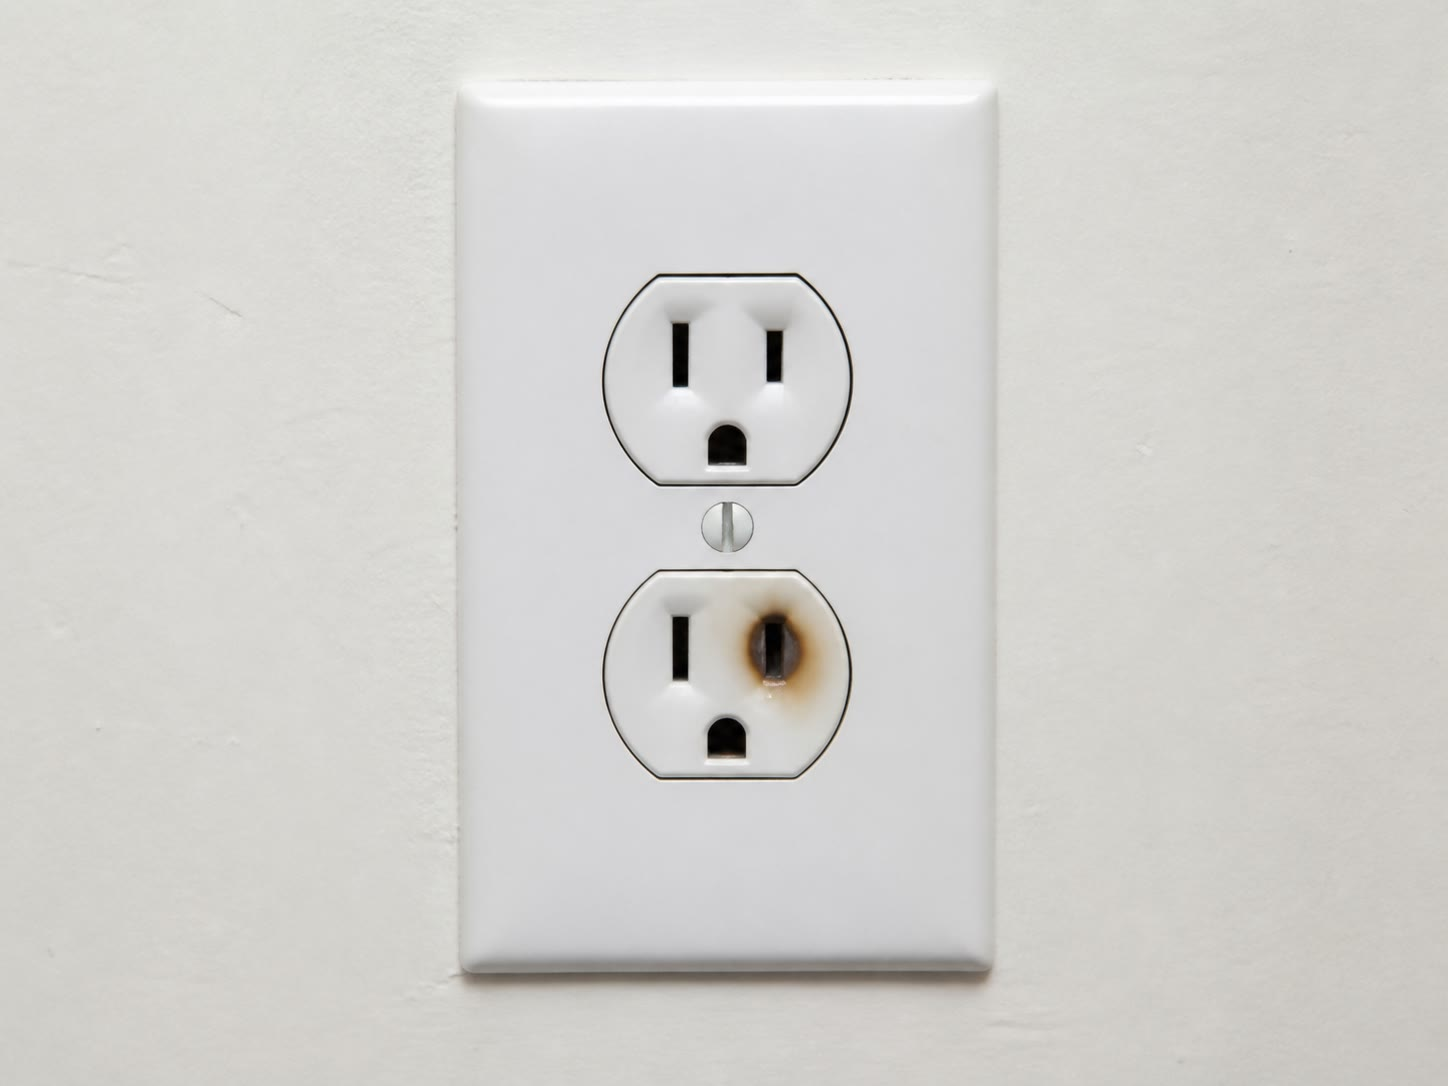
\includegraphics[width=0.45\linewidth]{images/book1/ai/g7-short-circuit-scorched.jpg}

{\small 故障留下的痕迹：过热电流烧焦了这个插座。这正是\omterm{def:g7:short-circuits-safety:fuse}{保险丝}与断路器要防止的危险。}
\end{omfigure}

\section{护卫装置}

\begin{definition}[保险丝]\label{def:g7:short-circuits-safety:fuse}
\emph{保险丝}\index{保险丝}是一种替你牺牲的护卫：一根
刻意做细的导线，与其所保护的电路\omterm{def:g4:series-circuits:series}{串联}，
当电流超过其额定值时熔断——从而切断电路——
奔涌的电流本可烧焦数米长的
房屋线路，如今却只烧毁三\omterm{def:g2:measuring-length:units}{厘米}长的牺牲导线，
它位于耐热的外壳之中。熔断的保险丝需要更换——
\emph{故障查明之后}——换上一根新的
额定值相同的保险丝。
\end{definition}

\begin{example}[断路器与保险丝：两位卫士，同一职责]\label{ex:g7:short-circuits-safety:breaker}
现代断路器履行\omterm{def:g7:short-circuits-safety:fuse}{保险丝}的职责却无需牺牲：它是一种
弹簧式\omterm{ex:g3:first-electric-circuit:switch}{开关}，在电流冲击时迅速断开，
拨动一下即可复位——但须在故障排除之后。无论\omterm{def:g7:short-circuits-safety:fuse}{保险丝}还是断路器，
其位置相同：\emph{\omterm{def:g4:series-circuits:series}{串联}}在其所保护的
\omterm{def:g5:series-parallel-circuits:parallel}{支路}上，使奔涌的电流必须经过它的关卡。
\omterm{def:g5:series-parallel-circuits:parallel}{并联}放置的卫士，只能看着电流
从另一条路径呼啸而过——纯属摆设。
\end{example}

\begin{example}[过载：礼貌的奔涌]\label{ex:g7:short-circuits-safety:overload}
并非每一次危险的奔涌都是\omterm{def:g7:short-circuits-safety:device}{短路}。一个多孔插座
同时为取暖器、水壶和烤面包机供电，
使其唯一的\omterm{def:g5:series-parallel-circuits:parallel}{支路}同时承载三股满负荷的电流——
每台用电器本身都无故障，但它们的总和构成过载，
像一台慢吞吞的烤面包机那样，使墙内线路逐渐发热。断路器因总电流而跳闸，理所当然。
家规：每个插座只接一台耗电发热的用电器；
多孔插座只用来接灯具和充电器，
不可用于私人厨房。
\end{example}

\begin{remark}[禁止的修理]\label{rem:g7:short-circuits-safety:nail}
这个古老的故事是真的，至今仍会致命：一户人家的\omterm{def:g7:short-circuits-safety:fuse}{保险丝}
屡屡熔断，有人便用钉子或硬币“修理”它——
那是一根粗壮、永不熔断的\omterm{def:g4:conductors-insulators:conductor}{导体}。症状被掩盖了；
病根依旧肆虐。下一次奔涌遇不到任何关卡，
屋里的电线本身就成了\omterm{def:g7:short-circuits-safety:fuse}{保险丝}——就在墙体之内。
切勿绕过卫士：屡屡熔断的\omterm{def:g7:short-circuits-safety:fuse}{保险丝}，
正是一位始终说实话的卫士。
\end{remark}

\begin{remark}[规则的最终形式]\label{rem:g7:short-circuits-safety:rules}
这本家庭用电“法典”，理由已然齐备：
切勿将\omterm{def:g3:first-electric-circuit:battery}{电池}的\omterm{def:g3:first-electric-circuit:battery}{接线柱}短接，汽车\omterm{def:g3:first-electric-circuit:battery}{电池}旁不可放扳手
（用金属使\omterm{def:g3:first-electric-circuit:battery}{电池}\omterm{def:g7:short-circuits-safety:device}{短路}即成焊接电弧）；每个插座只接
一台耗电发热的用电器（否则过载）；损坏的电线
必须报废（磨损的护套正在预演\omterm{def:g7:short-circuits-safety:device}{短路}）；水
与电源必须分开，双手务必干燥（人体决不可成为
旁路）；尊重卫士——只用规格相符的\omterm{def:g7:short-circuits-safety:fuse}{保险丝}，
故障须先排除，方可复位；插座本身，永远不可用于
插手指或做实验。
\end{remark}

\section{练习}

\begin{exercise}[$\star$]\label{exo:g7:short-circuits-safety:1}
叙述“无阻之路”命题。为何裸导线会
把奔涌的电流从\omterm{def:g3:first-electric-circuit:bulb}{灯泡}身边夺走？
\end{exercise}

\begin{exercise}[$\star$]\label{exo:g7:short-circuits-safety:2}
区分用电器的\omterm{def:g7:short-circuits-safety:device}{短路}与\omterm{def:g3:first-electric-circuit:battery}{电池}的\omterm{def:g7:short-circuits-safety:device}{短路}，
哪一种更严重？请说明理由。
\end{exercise}

\begin{exercise}[$\star$]\label{exo:g7:short-circuits-safety:3}
在安全演示中，\omterm{def:g3:first-electric-circuit:bulb}{灯泡} 2 为何会熄灭，
与此同时\omterm{def:g3:first-electric-circuit:bulb}{灯泡} 1 为何反而变亮？
\end{exercise}

\begin{exercise}[$\star$]\label{exo:g7:short-circuits-safety:4}
\omterm{def:g7:short-circuits-safety:device}{短路}时，导线为何会发热？日常生活中哪种用电器
有意利用同样的发热原理？
\end{exercise}

\begin{exercise}[$\star$]\label{exo:g7:short-circuits-safety:5}
什么是\omterm{def:g7:short-circuits-safety:fuse}{保险丝}，它牺牲了什么？为何它必须
与所保护的用电器\omterm{def:g4:series-circuits:series}{串联}？
\end{exercise}

\begin{exercise}[$\star$]\label{exo:g7:short-circuits-safety:6}
断路器比\omterm{def:g7:short-circuits-safety:fuse}{保险丝}有何改进？
两种卫士在复位或更换之前，必须先做什么？
\end{exercise}

\begin{exercise}[$\star$]\label{exo:g7:short-circuits-safety:7}
取暖器、水壶和烤面包机共用一个多孔插座。
导线没有裸露，用电器也无故障，断路器却跳闸。
请说出这一事件的名称，并解释\omterm{def:g5:series-parallel-circuits:parallel}{支路}的“抱怨”。
\end{exercise}

\begin{exercise}[$\star$]\label{exo:g7:short-circuits-safety:8}
为何用钉子“修理”\omterm{def:g7:short-circuits-safety:fuse}{保险丝}是家中最危险的行为之一？
此后什么会充当\omterm{def:g7:short-circuits-safety:fuse}{保险丝}？
\end{exercise}

\begin{exercise}[$\star\star$]\label{exo:g7:short-circuits-safety:9}
一根电线内的两根芯线，护套磨损，
在线缆内部相互接触——位于其所供电的\omterm{def:g3:first-electric-circuit:bulb}{灯泡}上游。请诊断：
属于哪一种\omterm{def:g7:short-circuits-safety:device}{短路}，\omterm{def:g3:first-electric-circuit:bulb}{灯泡}会怎样，
\omterm{def:g5:series-parallel-circuits:parallel}{支路}上的卫士又会做什么？
\end{exercise}

\begin{exercise}[$\star\star$]\label{exo:g7:short-circuits-safety:10}
在双\omterm{def:g3:first-electric-circuit:bulb}{灯泡}演示中，若改将旁路导线
跨接在\emph{两只}\omterm{def:g3:first-electric-circuit:bulb}{灯泡}上（即从\omterm{def:g3:first-electric-circuit:bulb}{灯泡} 1 之前
接到\omterm{def:g3:first-electric-circuit:bulb}{灯泡} 2 之后），请预测会发生什么，此时应适用哪一个定义，
实验者为何不可尝试？
\end{exercise}

\begin{exercise}[$\star\star$]\label{exo:g7:short-circuits-safety:11}
圣诞节清晨之谜：祖母的一串
\omterm{def:g4:series-circuits:series}{串联}小彩灯中，有一只\omterm{def:g3:first-electric-circuit:bulb}{灯泡}在熄灭时，内部支撑线已熔接在一起，
使其自身\omterm{def:g7:short-circuits-safety:device}{短路}。与通常的悲剧相反，
这串彩灯的\emph{其余部分仍然亮着}，且略微更亮。
请解释原因，并说明其余\omterm{def:g3:first-electric-circuit:bulb}{灯泡}
正在悄然酝酿什么。
\end{exercise}

\begin{exercise}[$\star\star\star$]\label{exo:g7:short-circuits-safety:12}
为一间小车间设计防护方案：三条\omterm{def:g5:series-parallel-circuits:parallel}{并联}的\omterm{def:g5:series-parallel-circuits:parallel}{支路}
（照明；电动工具；\omterm{def:g3:first-electric-circuit:battery}{电池}充电器）共用一个电源。
设置卫士与\omterm{ex:g3:first-electric-circuit:switch}{开关}；选出哪些\omterm{def:g5:series-parallel-circuits:parallel}{支路}应单独配备卫士，并说明理由；
并在\omterm{def:g7:short-circuits-safety:fuse}{保险丝}抽屉上方写一份两行告示，
概括
\cref{rem:g7:short-circuits-safety:nail}的要点。
\end{exercise}

\section{周末问题：火灾调查员的报告}

\begin{problem}[{周末问题——公寓火灾之后；
调查员读懂了电线的“供词”；三处故障，
一个教训}]\label{pb:g7:short-circuits-safety:1}
没有人受伤——一家人外出了——但厨房的墙
已被烧焦，调查员必须依据
证据还原那一夜的情况。你带着她的笔记本。

\medskip\noindent\textbf{第一部分——读懂废墟。}
\begin{enumerate}
  \item 证物一：一个多插座，给取暖器、水壶
        和深油炸锅供电，其塑料外壳已半\omterm{def:g6:water-states:changes}{熔化}，其中
        没有任何裸露的导线。说出这件证物所提示的故障，
        并说明为何它不需要“恶毒的导线”也能形成。
  \item 证物二：橱柜后面的一根电线，被宠物
        咬过，两根导线在咬痕处
        相互接触。说出这种故障，并说明从接触的那一刻起，
        电流走向了何处。
  \item 证物三，也是最具决定性的一件：在\omterm{def:g7:short-circuits-safety:fuse}{保险丝}盒中，厨房\omterm{def:g5:series-parallel-circuits:parallel}{支路}的
        \omterm{def:g7:short-circuits-safety:fuse}{保险丝}管内装的是——一条卷起的
        锡箔纸条。说明这种“修理”对该\omterm{def:g5:series-parallel-circuits:parallel}{支路}的
        保护作用造成了什么影响。
  \item 将三件证物串成一个合理的经过：哪一处故障
        最先出现，真正的\omterm{def:g7:short-circuits-safety:fuse}{保险丝}在证物三出现之前对它做了什么，
        以及为何最后那一夜以火灾收场，
        而不是厨房只是断电变暗。
\end{enumerate}

\medskip\noindent\textbf{第二部分——物理证词。}
\begin{enumerate}[resume]
  \item 法庭问道：为什么\omterm{def:g7:short-circuits-safety:device}{短路}或过载的电线会
        \emph{发热}？请举出一种日常器具，它证明
        电流发热是可以驾驭的——而此处缺少的是
        什么。
  \item 为什么\omterm{def:g7:short-circuits-safety:fuse}{保险丝}要特意做得很细？请解释“一个
        为你献身的护卫”这一说法。
  \item 锡箔纸条导电性能极佳。恰恰
        \emph{正因为}如此，它作为护卫却失效了。请为
        陪审团解开这个小小的矛盾。
  \item 取暖器单独使用时是安全的，水壶单独使用时是安全的，
        油炸锅单独使用时也是安全的。请用一句话说明，三者
        各自安全，合在一起为何成了一处危险。
\end{enumerate}

\medskip\noindent\textbf{第三部分——裁决与
教训。}
\begin{enumerate}[resume]
  \item 调查员必须按“责任轻重”对三处故障排序：
        过载、被咬坏的电线、锡箔纸。哪一处
        使意外变成了灾难？为什么？
  \item 家人问道：火灾当夜若装有合格的\omterm{def:g7:short-circuits-safety:fuse}{保险丝}，
        结果会怎样？请带他们逐分钟地
        讲述这一过程。
  \item 建议重新布线：取暖器、水壶和
        油炸锅现在应如何供电，多插座今后应
        遵守怎样的常规规定？
  \item 以调查员的三句话总结结束报告：
        施害者的手法、护卫的职责，以及
        绝不能即兴处理的那一项修理。
\end{enumerate}
\end{problem}
